\section{Network Scan}

\subsection{How we scanned}
\begin{enumerate}
    \item Connect to the jump host:
    \begin{lstlisting}[language=bash,numbers=none]
ssh sse_team16@10.10.20.100 -p 13316
    \end{lstlisting}

    \item Find the configured IP addresses and the available networks on the jump host
    \begin{lstlisting}[language=bash,numbers=none]
$ ip add
1: lo: <LOOPBACK,UP,LOWER_UP> mtu 65536 qdisc noqueue state UNKNOWN group default qlen 1000
    link/loopback 00:00:00:00:00:00 brd 00:00:00:00:00:00
    inet 127.0.0.1/8 scope host lo
        valid_lft forever preferred_lft forever
    inet6 ::1/128 scope host
        valid_lft forever preferred_lft forever
129: eth0@if4: <BROADCAST,MULTICAST,UP,LOWER_UP> mtu 1500 qdisc noqueue state UP group default
    link/ether 02:42:c0:a8:2d:50 brd ff:ff:ff:ff:ff:ff link-netnsid 0
    inet 192.168.45.80/24 brd 192.168.45.255 scope global eth0
        valid_lft forever preferred_lft forever
    inet6 fdcb:c447:e992:3553:1005::b0/120 scope global nodad
        valid_lft forever preferred_lft forever
    inet6 fe80::42:c0ff:fea8:2d50/64 scope link
        valid_lft forever preferred_lft forever
132: eth1@if133: <BROADCAST,MULTICAST,UP,LOWER_UP> mtu 1500 qdisc noqueue state UP group default
    link/ether 02:42:ac:12:00:74 brd ff:ff:ff:ff:ff:ff link-netnsid 0
    inet 172.18.0.116/16 brd 172.18.255.255 scope global eth1
        valid_lft forever preferred_lft forever
    \end{lstlisting}

    \item Scan the IPv4 networks for hosts and show their open ports
    \begin{lstlisting}[language=bash,numbers=none]
nmap -PE 192.168.45.0/24
nmap -PE 172.26.0.0/16
    \end{lstlisting}
    I scan the whole 172.26.0.0/16 subnet to figure out the network address of 172.26.Z.0/24.
    After the scan, I figured out that the network that I am searching for is 172.26.66.0/24.

    \item Scan the IPv6 networks for hosts
    \begin{lstlisting}[language=bash,numbers=none]
nmap -PE -6 fdcb:c447:e992:3553:1000::/120 # empty
nmap -PE -6 fdcb:c447:e992:3553:1001::/120 # empty
nmap -PE -6 fdcb:c447:e992:3553:1002::/120 # empty
nmap -PE -6 fdcb:c447:e992:3553:1003::/120 # empty
nmap -PE -6 fdcb:c447:e992:3553:1004::/120 # empty
nmap -PE -6 fdcb:c447:e992:3553:1005::/120
nmap -PE -6 fdcb:c447:e992:3553:1006::/120
nmap -PE -6 fdcb:c447:e992:3553:1007::/120
nmap -PE -6 fdcb:c447:e992:3553:1008::/120 # empty
nmap -PE -6 fdcb:c447:e992:3553:1009::/120 # empty
nmap -PE -6 fdcb:c447:e992:3553:100a::/120 # empty
nmap -PE -6 fdcb:c447:e992:3553:100b::/120 # empty
nmap -PE -6 fdcb:c447:e992:3553:100c::/120 # empty
nmap -PE -6 fdcb:c447:e992:3553:100d::/120 # empty
nmap -PE -6 fdcb:c447:e992:3553:100e::/120 # empty
nmap -PE -6 fdcb:c447:e992:3553:100f::/120 # empty
    \end{lstlisting}
\end{enumerate}

After I have done the tasks from above, I have a full list of the hosts that are available on the needed networks
and I can go ahead and scan for more specific information

\begin{enumerate}
    \item Scan all open ports of the found hosts in 172.26.66.0/24:
    \begin{lstlisting}[language=bash,numbers=none]
nmap -p- 172.26.66.X
    \end{lstlisting}
    Where X builds to one of the IPs from the table below.

    \item Go through the hosts from the list and scan for their OS and service version
    \begin{lstlisting}[language=bash,numbers=none]
nmap -A X # where X is an IPv4 address from the table
nmap -A6 X # where X is an IPv6 address from the table
    \end{lstlisting}

    \item Trace the route to a host in 172.26.66.0/24 to determine our default gateway
    \begin{lstlisting}[language=bash,numbers=none]
$ traceroute 172.26.66.1

traceroute to 172.26.66.1 (172.26.66.1), 64 hops max
    1   192.168.45.1  0.594ms  0.164ms  0.112ms
    2   172.26.66.1  0.629ms  0.248ms  0.205ms
    \end{lstlisting}

    \item We can call this command after every scan to get the MAC addresses of the found hosts
    (will work only in the same broadcast domain, we cannot determine the MAC addresses of hosts in remote networks)
    \begin{lstlisting}[language=bash,numbers=none]
ip neigh # get our neighbours as the arp command is not available
    \end{lstlisting}

    \item I then went and scanned all the ports of the found IPv4 and IPv6 addresses and compared them
    to determine on which interfaces the services were running
    \begin{lstlisting}[language=bash,numbers=none]
nmap -p- X # X is an IPv4 address from below
nmap -p- -6 Y # Y is an IPv6 address from below
    \end{lstlisting}

\end{enumerate}

\subsection{Results}

The results that I obtained are documented in the table below (a little zoom may be needed :)).

NOTE:
\begin{itemize}
    \item 22/tcp4 - means that the host listens on this port on the IPv4 interface
    \item 22/tcp6 - means that the host listens on this port on the IPv6 interface
    \item 22/tcp  - means that the host listens on this port on both IPv4 and IPv6 interfaces
\end{itemize}
\begin{center}
    \resizebox{\textwidth}{!}{
        \begin{tabular}{| c | c | c | c | c | c | c |}
        \hline
        Hostname (DNS) & IPv4 address & IPv6 address & MAC address & OS & Open Ports & Suspected functionality \\ [0.5ex]
        \hline\hline
        sun.local.vienna.essecorp.invalid       & 192.168.45.1   & fdcb:c447:e992:3553:1005::1  & 00:1b:d2:0d:84:44 & Linux (Debian) & 22/tcp (ssh), 10050/tcp (zabbix-agent) & gateway \\
        \hline
        venus.local.vienna.essecorp.invalid     & 192.168.45.4   & fdcb:c447:e992:3553:1005::4  & 00:1b:d2:b3:43:62 & Unix-like (dns is dnsmasq) & 53/tcp4 (dns) & dns \\
        \hline
        saturn.local.vienna.essecorp.invalid    & 192.168.45.21  & fdcb:c447:e992:3553:1005::5  & 00:1b:d2:1a:c9:75 & Unix-like (mail servers - dovecot, exim) & 25/tcp (smtp), 110/tcp (pop3), 143/tcp (imap) & mail server \\
        \hline
        mars.local.vienna.essecorp.invalid      & 192.168.45.56  & fdcb:c447:e992:3553:1005::16 & 00:1b:d2:81:54:c3 &  Unix-like (tcp6 proxy is tinyproxy) & 1080/tcp4 (socks), 8080/tcp6 (proxy) & proxy \\
        \hline
        jupiter.local.vienna.essecorp.invalid   & 192.168.45.99  & fdcb:c447:e992:3553:1005::2b & 00:1b:d2:80:96:13 & Unix-like (server is CUPS) & 631/tcp (ipp) & print server \\
        \hline
        mercury.local.vienna.essecorp.invalid   & 192.168.45.202 & fdcb:c447:e992:3553:1005::55 & 00:1b:d2:fe:bc:17 & ? & N/A & ? \\
        \hline
        neptune.local.vienna.essecorp.invalid   & 192.168.45.204 & fdcb:c447:e992:3553:1005::4f & 00:1b:d2:1e:cd:a0 & Linux (Debian) & 139/tcp (netbios-ssn), 445/tcp (smb) & file server \\
        \hline
        ws00-ws28.local.vienna.essecorp.invalid & 192.168.45.64-92 & fdcb:c447:e992:3553:1005::a0 - bc & N/A & Linux (Debian) & 22/tcp (ssh) & team machines \\
        \hline
        tauceti.dmz.vienna.essecorp.invalid     & 172.26.66.1    & fdcb:c447:e992:3553:1006-7::1 & N/A & Linux (Debian) & 22/tcp (ssh), 10050/tcp (zabbix-agent) & gateway \\
        \hline
        pluto.dmz.vienna.essecorp.invalid       & 172.26.66.12   & N/A & N/A & ? (nginx, mariadb are multi-platform) & 80/tcp4 (http) 3306/tcp4 (mysql) & web server with mysql database \\
        \hline
        aegaeon.dmz.vienna.essecorp.invalid     & 172.26.66.15   & N/A & N/A & Unix-like (ftp is vsftpd) & 21/tcp4 (ftp), 1194/tcp4 (openvpn) & FTP and VPN server \\
        \hline
        ophelia.dmz.vienna.essecorp.invalid     & 172.26.66.27   & N/A & N/A & Unix-like (smtp server is exim) & 25/tcp4 (smtp) & mail server \\
        \hline
        makemake.dmz.vienna.essecorp.invalid    & 172.26.66.253  & fdcb:c447:e992:3553:1006::fd & N/A & Linux(Debian) & 22/tcp (ssh), 10050/tcp (zabbix-agent) & ? \\
        \hline
        sirius.extra.vienna.essecorp.invalid    & N/A & fdcb:c447:e992:3553:1007::7f & N/A & ? (nginx is multi-platform) & 80/tcp6 (http), 443/tcp6 (https) & web server \\
        \hline
        procyon.extra.vienna.essecorp.invalid   & N/A & fdcb:c447:e992:3553:1007::9a & N/A & Linux (as reported from nmap) & 7/tcp6 (echo), 9/tcp6 (discard), 13/tcp6 (daytime) 19/tcp6 (chargen), 37/tcp6 (time) & test server? \\
        \hline
    \end{tabular}
    }
\end{center}

\subsection{Network Diagram}
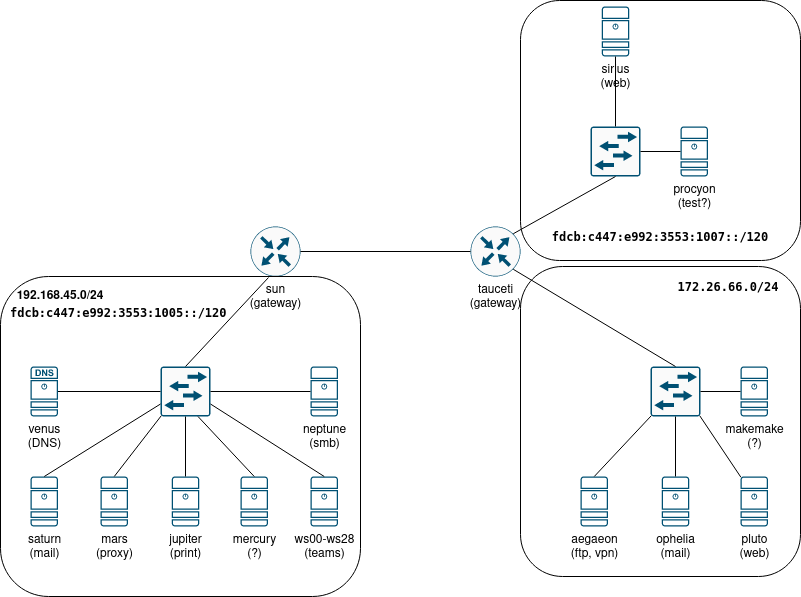
\includegraphics[scale=0.6]{imgs/sse-netscan.png}
